\subsection{Première partie : L'automate}
    \subsubsection{Automate : Généralités}
        \paragraph*{}
        L'automate sur lequel j'ai travaillé était un automate venant de chez Schneider Electric comme abordé dans la partie \ref{part-automate}. Il est accessible en se connectant via le réseau local et on communique avec l'automate grâce au protocole de communication ModBus. Ce protocole a été créé par l'entreprise Modicon en 1979. Cette société a ensuite été achetée en 1996 par Schneider Electric. Il est utilisé pour les automates programmables et s'applique sur la couche applicative (Niveau 7 du modèle $OSI$\footnote{Le modèle $OSI$ est une norme de communication de tous les systèmes informatiques proposé par l'$ISO$.}). Ce protocole est basé sur une structure hiérarchisée comme par exemple : Maitre/Esclaves ou Client/Serveurs. Pour mon stage, j'utilisais ce protocole en mode TCP/IP et donc Client/Serveur. Le client était déterminé par l'ordinateur sur lequel je travaillais et c'est via cet ordinateur que j'accédais à l'automate via des lectures et écritures dans le serveur qui était l'automate. Le serveur est identifié par une adresse IP et un numéro de port sur lequel il attend les demandes de connexion (port 502 par défaut). Le port du client sera lui toujours supérieur à 1024 afin de ne pas se superposer avec les ports définis pour le système et sera différent pour chaque client connecté simultanément.
        
        \label{part:unityPro}
        Pour le programmer, récupérer les variables, les registres ou modifier le fonctionnement, il est nécessaire d'utiliser le logiciel \textsc{Unity Pro XLS}  et de programmer l'automate en Grafcet (GRAphe Fonctionnel de Commande Étapes / Transitions) ou en C. Ce langage de programmation est un mode de représentation d'un automatisme très bien adapté aux systèmes séquentiels. Il est possible de comparer le Grafcet au modèle mathématique des réseaux de Petri. Le Grafcet est un langage graphique qui représente le fonctionnement d'un automate par une suite d'étapes associées à des actions et des transitions entre chaque étape (voir l'exemple à la figure \ref{fig:grafcet}).
        
        \begin{figure}[H]
            \centering
            \begin{frame}{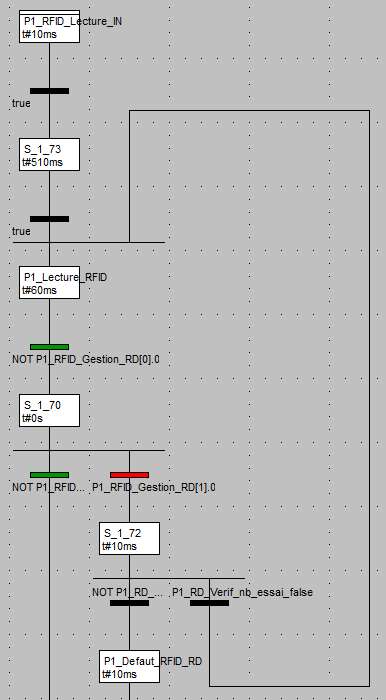
\includegraphics[width=0.5\textwidth]{image/grafcet.png}}
            \end{frame}
            \caption{\label{fig:grafcet}Exemple de code Grafcet}
        \end{figure}
        
        \paragraph*{}
        Les automates de la plateforme sont composés de registres. Chaque registre est déterminé par son adresse. Il y a plusieurs types de registre :
        
        \begin{itemize}
        \item \%I : représente une entrée (Input); elle est mise à jour dans la mémoire en début de tâche ou quand l'automate est en mode RUN ou STOP. Exemple : \textit{\%I0.2.39.0} correspond à la valeur d'entrée pour la présence du flacon sur la palette.
        \item \%Q : représente une sortie ; elle est mise à jour à la fin de la tâche, uniquement lorsque l'automate est en mode RUN. Exemple : \textit{\%Q0.3.16.0}
        \item \%M : représente un mot de taille 1 (type bit mémoire). Exemple : \textit{\%M103} correspond à la présence d'une palette ou non sous le récipient à bille n°1.
        \item \%MW : représente un mot d'une taille \textsc{N} (type mot mémoire). Exemple : \textit{\%MW150} correspond à la lecture de la puce RFID au niveau du poste 1 (récipient à bille).
        \end{itemize}
        
        Il existe d'autres types de registres mais je ne les ai pas utilisés, voir ils pouvaient ne pas être utilisé du tout dans la base de registre à ma disposition.
        
        Dans mon cas, j'ai dû lire les valeurs des registres seulement dans les registres de type \textit{\%M} et \textit{\%MW}.
    
    
    \subsubsection{Automate : Récupération des valeurs des registres}
    \label{part:readReg}
        \paragraph*{}
        J'ai créé un programme Java me permettant, via une interface homme/machine (voir figure \ref{fig:ihmJava}), de récupérer les valeurs des registres de l'automate depuis l'ordinateur qui sert de Client. J'ai inscrit des valeurs par défaut dans le code afin de simplifier et accélérer l'exécution du programme lorsque l'on désire faire plusieurs relevés avec peu de délai entre chaque exécution.
        
        \paragraph*{}
        Les valeurs que je récupère depuis les registres de l'automate sont également accessibles via le logiciel \textit{Unity Pro XLS}, comme dit dans la partie \ref{part:unityPro}. Comme on peut voir à la figure \ref{fig:regUnity}, le registre s'appelant 'P1\_Presence \_palette\_img' correspond au registre \textit{\%M103} qui est de taille 1; quant au deuxième registre se nommant 'P1\_RFID\_Gestion\_RD', il correspond au tableau de registre de taille 4 \textit{\%MW150} et c'est seulement la première valeur qui change à chaque fois que la palette fait un tour sur le convoyeur visible à la figure \ref{fig:module-plateforme}.
        
        \begin{figure}[H]
            \centering
            \begin{frame}{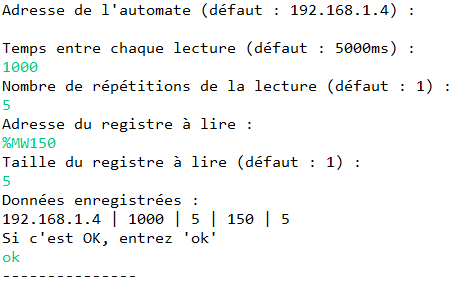
\includegraphics[width=0.9\textwidth]{image/ihmJava.png}}
            \end{frame}
            \caption{\label{fig:ihmJava}Aperçu de l'$IHM$  textuelle du programme Java}
        \end{figure}
        
        \begin{figure}[H]
            \centering
            \begin{frame}{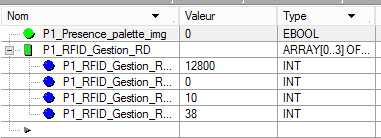
\includegraphics[width=1\textwidth]{image/regUnity.png}}
            \end{frame}
            \caption{\label{fig:regUnity}Aperçu du contenu des registres sur le logiciel \textit{Unity Pro XLS}}
        \end{figure}
        
        \paragraph{Code Java}
        \label{part:progJava}
            \paragraph*{}
            Afin de programmer l'application, il me fallait me connecter à l'automate, renseigner l'adresse du registre, le type de registre et la taille du registre à lire, le nombre de fois que l'on veut lire ce registre et à quel intervalle.
            
            Les valeurs par défaut sont inscrites dans le code et s'affichent lors de l'exécution. Pour modifier une valeur par défaut il suffit de rentrer une valeur au clavier, elle apparaitra en vert (voir image \ref{fig:ihmJava}) dans la console.
            
            Une fois les valeurs rentrées lors de l'exécution, un message de confirmation apparaît afin de bien vérifier les valeurs et qui permet de corriger une valeur s'il y a une erreur au lieu de tout relancer. Une fois la confirmation faite, le programme se lance.
            
            \paragraph*{}
            Tout d'abord, l'application lance la connexion sur l'adresse de l'automate donnée dans les valeurs précédentes et sur le port 502 qui est celui par défaut (voir le détail dans la partie \ref{part:connectAuto}). Si la connexion est réussie, il affichera \textit{Client connecté} sinon il affichera un message d'erreur correspondant au type d'erreur rencontrée comme par exemple un client déjà connecté à l'automate, une connexion impossible (cable ethernet débranché par exemple).
            
            Ensuite, si la connexion avec l'automate est réalisée, la lecture de la variable peut se faire (voir la partie \ref{part:lectureReg} pour plus de détails).
            
            Enfin, il y a déconnexion entre le serveur et le client et affichage du message de retour : \textit{Client déconnecté} ou \textit{Client non déconnecté}.
            
            \paragraph*{}
            Dans les prochaines pages, des morceaux de code seront présentés. Le code est mis tel que je l'ai dans mon programme. Des parties peuvent être abordées sans expliquer totalement le code mis; mais les parties non expliquées le seront dans les paragraphes suivants.
        
        \paragraph{Connexion à l'automate}
        \label{part:connectAuto}
            \paragraph*{}
            Pour connecter le client au serveur, il fallait établir un protocole de communication ModBus. J'ai ainsi, dans mon programme Java, incorporé une librairie qui gère le protocole ModBus afin de communiquer avec l'automate. Pour se faire, j'ai utilisé la librairie \textit{j2mod}\cite{j2mod}.
            
            Cette librairie est très simple d'utilisation et possède un tutoriel sur GitHub afin de démarrer et commencer à communiquer\cite{j2modGithub}.
            
            Afin de lancer la connexion avec le serveur, il suffit d'appeler le constructeur puis une fonction comme on peut voir à la ligne \textit{4} et \textit{5} du bloc de code \ref{code:connectServeur} en annexe 2. Le constructeur prend en paramètre l'adresse IP du serveur. Dans mon cas, j'ai stocké cette adresse dans un attribut de la classe et donc je passe seulement cet attribut au constructeur. La fonction générale que l'on peut voir sur le bloc \ref{code:connectServeur} en annexe 2 renvoie, si la connexion s'est bien exécutée ou non afin d'afficher à l'utilisateur, un message visuel dans la console.
    
        \paragraph{Lecture des registres}
        \label{part:lectureReg}
            \paragraph*{}
            Une fois que la connexion est faite entre le Client et le Serveur, il est possible de récupérer la valeur d'un registre. Dans mon code j'ai créé une fonction principale qui va lire un registre de taille \textit{N}. La petite difficulté est qu'il y a deux types de registres différents à lire et de tailles différentes. Un des registres sera toujours de taille 1 et l'autre est un tableau de \textit{N cases}. Ainsi, la fonction principale, appelée \verb|readVar()|, permet la séparation des appels selon le type de registre et permet également la répétition de la lecture selon le nombre de répétitions et le délai demandé par l'utilisateur.
            
            \paragraph*{}
            Une fois que le type de registre est connu du programme, il peut appeler la fonction correspondante afin de lire le contenu selon la taille. La taille du registre influera sur la fonction de la librairie. Une fois l'appel de la fonction fait, le résultat est affiché dans la console pour l'utilisateur.
            
        
        \paragraph{Améliorations possibles}    
            \paragraph*{}
            Les améliorations possibles de cette partie sont de formater le code professionnellement. Par exemple, en gérant les exceptions dans une classe séparée du code et non pas directement dans le code comme actuellement.
        
        \paragraph{Résultat}    
            \paragraph*{}
            Comme il est possible de voir sur les blocs \ref{code:execM} et \ref{code:execMW} en Annexe 2, l'exécution du programme se fait via une interface minimale textuelle et affiche les résultats à la ligne à chaque lecture.


    \subsubsection{Automate : Enregistrement des valeurs dans une base de données}
        \paragraph*{}
        Dans cette nouvelle sous-partie, je vais évoquer les améliorations du programme que j'ai abordé dans la partie \ref{part:progJava}. Le but principal du projet est, rappelons le, la surveillance d'une plateforme de manière automatisée avec traitement et analyse des erreurs survenues.
        
        Ainsi, pour se faire, il est nécessaire de vérifier en continu les valeurs des registres comme nous l'avons abordé dans la partie \ref{part:readReg}. Puis ensuite, de stocker ces valeurs récupérées dans une base de données qui sera accessible au drone afin d'analyser ces valeurs et détecter une potentielle erreur qui serait survenue avant d'intervenir (voir la partie \ref{part:drone}).
        
        \paragraph*{}
        C'est pourquoi, j'ai itéré une première fois la version du programme Java de la partie \ref{part:readReg} en y ajoutant cette fois une partie de stockage et lecture de la base de données. La base de données que nous utilisons est une base de données en local directement installée sur l'ordinateur "Client", elle est de type 'Microsoft SQL Server 2014' et on y accède via \textit{localhost} sur le port 49190.
        
        \paragraph{Le Driver JDBC}
            \paragraph*{}
            Pour travailler avec une base de données en Java, il est nécessaire d'utiliser un driver qui permettra de faire le lien entre la base de données et l'application Java. Le driver est dépendant du type de base de données. Étant donné que j'utilise une base de données de type 'Microsoft SQL Server 2014', je suis allé récupérer le driver sur le site de Microsoft\cite{msDriverSQL}.
        
        \paragraph{Programmation et exécution de l'application}
            \paragraph*{}
            Une fois le driver installé selon la version Java du programme (version 8 de Java pour ma part), il faut indiquer dans les attributs de connexion l'URL avec une forme précise : \textit{jdbc:sqlserver://localhost//SQL2014:49190;}. Ensuite dans la même chaine de caractère, on indique le nom de la base (\textit{sensorData} pour moi), l'utilisateur et le mot de passe. Cette chaine de caractère donne donc pour moi : \textit{jdbc:sqlserver://localhost//SQL2014:49190; database=sensorData; user=XXX; password=XXX;}.
            
            Le programme se connecte à la base de données via cette chaine de caractère puis ensuite, il est possible de lancer des requêtes SQL tel que des \textit{INSERT}, \textit{SELECT} ou \textit{DELETE}. J'ai créé des fonctions permettant de gérer les requêtes SQL de type \textit{INSERT} et \textit{SELECT}.
            
            La fonction d'insertion (voir bloc de code n°\ref{code:fctSQL} en Annexe 2) prend en paramètre une chaine de caractère et un objet. La chaine de caractère servira à déterminer le nom du registre à insérer et l'objet est une valeur numérique qui correspondra à la valeur du registre au moment de la lecture.
            
            La fonction de sélection prend en paramètre également une chaine de caractère correspondant à ce que l'on veut récupérer de la base de données (tout, une colonne, ...) et une chaine de caractère correspondant aux options possible dans une requête SQL.
            Les options peuvent être par exemple \textit{WHERE}, \textit{ORDER BY}, \textit{GROUP BY}, etc. Ces fonctions sont appelées dans les fonctions de lecture des variables comme on peut voir sur le bloc de code \ref{code:readVar} en Annexe 2 pour la fonction \textit{select()} ou sinon dans les sous-fonctions de lecture spécifique (voir le bloc de code \ref{code:readAddr} en Annexe 2) pour la fonction \textit{insert()}.
            
            
            
            \paragraph*{}
            Un exemple d'appel de ces fonctions peut être :
            \begin{lstlisting}[language=Java, caption=Exemple d'utilisation des fonctions SQL]
requete.insert("MW150", 1);
requete.select("*", "WHERE registerName = 'MW150'");\end{lstlisting}
            
            \paragraph*{}
            Ce qui équivaut à faire en SQL :
            \begin{lstlisting}[language=SQL, caption=Équivalent SQL]
INSERT sensorValue (registerName, registerValue) VALUES ('MW150','1');
SELECT * FROM sensorValue WHERE registerName = 'MW150'");\end{lstlisting}
        
        
        \paragraph{Résultat}    
        \paragraph*{}
        Comme il est possible de voir sur le bloc \ref{code:execSQL} en Annexe 2 et la figure \ref{fig:saveSQL}, l'exécution du programme et l'enregistrement dans la base de données se fait bien. Il est possible de lire les données des registres de l'automate et de les sauvegarder dans la base de données.
        
        
        \begin{figure}[H]
            \centering
            \begin{frame}{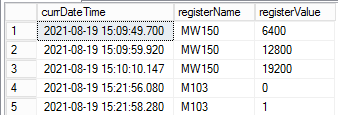
\includegraphics[width=1\textwidth]{image/exempleSQLSave.png}}
            \end{frame}
            \caption{\label{fig:saveSQL}Capture d'écran de la base de données}
        \end{figure}
    
    \subsubsection{Conclusion partielle}
        \paragraph*{}
        L'objectif de cette partie était de se connecter à l'automate, lire les valeurs des registres puis sauvegarder cette valeur dans une base de données afin que le drone, que l'on abordera dans la partie suivante, puisse accéder à cette valeur et détecter s'il y a une anomalie qui s'est produite ou non.
        
        \paragraph*{}
        Pour se faire, j'ai ainsi créé un programme Java qui se connecte à l'automate selon des paramètres donnés par l'utilisateur. Dans un second temps, il va lire la valeur du registre ou les valeurs si le registre demandé est un tableau. Enfin pour terminer, le programme sauvegarde la valeur du registre lu dans une base de données de type 'Microsoft SQL Server 2014' afin que la valeur soit accessible plus tard par le drone ou par un utilisateur de la chaine de production.